% Drawing 146/07-4 -- folder 146, batch 07, archive page 127 (PDF page 128).
% Transcription: un graphe à trois sommets $g_1$, $g_2$, $g_3$ : $g_1$ porte trois arêtes libres et deux arêtes vers $g_2$, $g_2$ porte une boucle et une arête libre et est relié à $g_3$, qui porte deux arêtes libres.
% Kind: stable graph (MD graph) with genus labels. Method 3 (encoded, rendered from the data). Status: ok.
% Notes: Three vertices g1, g2, g3 (genera named, not numbered): g1 with three legs and two edges to g2, g2 with a loop and one leg, joined to g3 with two legs. Encoded with symbolic genera: b1 = 2, nu = 6, type (2 + g1 + g2 + g3, 6); every vertex has valence >= 3, so it is stable whatever the genera. Matches the transcription.
% Coordinates: 1 unit = 1 mm = 1/100 of the crop width (bbox in page fractions: [0.75, 0.44, 0.91, 0.525]).
% Redrawn by Claude (claude-opus-5-5), issue #73 pilot, 2026-11-07; not checked by a human; not compiled (no TeX in the session).
% Rights: reproduces part of the work -- behind RENDER_TRANSCRIPTS, never published by itself.
\documentclass[tikz,border=3pt]{standalone}
\usepackage{amsmath,amssymb}
\usetikzlibrary{patterns,arrows.meta}
\tikzset{pencil/.style={black!45}, struck/.style={black!35}, mark/.style={circle,draw,inner sep=1.3pt}, pt/.style={circle,fill,inner sep=0.9pt}, opt/.style={circle,draw,fill=white,inner sep=1.1pt}}
\begin{document}
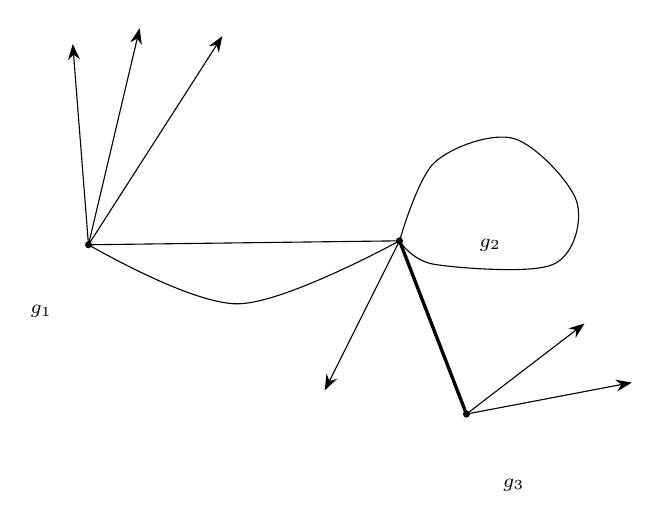
\begin{tikzpicture}[x=1mm,y=1mm,line cap=round,line join=round,font=\scriptsize]
\draw[-{Stealth[length=2mm]}] (21,-38.5) -- (19,-13);
\draw[-{Stealth[length=2mm]}] (21,-38.5) -- (27.5,-11);
\draw[-{Stealth[length=2mm]}] (21,-38.5) -- (38,-12);
\draw (21,-38.5) -- (60.5,-38);
\draw plot[smooth, tension=0.55] coordinates {(21,-38.5) (40,-46) (60.5,-38)};
\draw plot[smooth, tension=0.55] coordinates {(60.5,-38) (65,-28) (75,-25) (83,-33) (80,-41) (65,-41) (60.5,-38)};
\draw[-{Stealth[length=2mm]}] (60.5,-38) -- (51,-57);
\draw[very thick] (60.5,-38) -- (69,-60);
\draw[-{Stealth[length=2mm]}] (69,-60) -- (84,-48.5);
\draw[-{Stealth[length=2mm]}] (69,-60) -- (90,-56);
\node[pt] at (21,-38.5) {};
\node[pt] at (60.5,-38) {};
\node[pt] at (69,-60) {};
\node[inner sep=1pt] at (15,-47) {\scriptsize $g_1$};
\node[inner sep=1pt] at (72,-38.5) {\scriptsize $g_2$};
\node[inner sep=1pt] at (75,-69) {\scriptsize $g_3$};
\end{tikzpicture}
\end{document}
